\documentclass[eng,openany]{mgr}
\usepackage{listings}
\usepackage[english]{babel}
\usepackage{graphicx}
\usepackage{hyperref}
\usepackage{tabularx,colortbl} 
\usepackage{rotating}
\usepackage[utf8]{inputenc} 
\usepackage{amssymb}
\setlength\parindent{24pt}
\usepackage[parfill]{parskip}
\usepackage[table,kernelfbox,hyperref]{xcolor}
\usepackage{fancyhdr}
\usepackage{gauss}
%\usepackage[colorinlistoftodos]{todonotes}

\hypersetup{colorlinks=true}
\hypersetup{xurlbordercolor=red!70!black}
\hypersetup{xlinkbordercolor=blue!70!black}
\hypersetup{linkcolor=blue!60!black}
\hypersetup{urlcolor=red!50!black}
\hypersetup{citecolor=green!30!black}
\rfoot{Page \thepage}
\renewcommand\lstlistlistingname{List of Listings}
\newcommand{\linia}{\rule{\linewidth}{0.4mm}}

\definecolor{listlightgray}{gray}{0.93}

\newcommand{\lstsetmylst} {
\lstset{frame = tb,
breaklines=true,
framerule = 0.25pt,
float,
fontadjust,
backgroundcolor={\color{listlightgray}},
basicstyle = {\ttfamily\footnotesize},
identifierstyle = {\ttfamily},
stringstyle = {\ttfamily},
showstringspaces = false,
showtabs = false,
numbers = left,
numbersep = 6pt,
tabsize = 4,
language=C,
floatplacement=!h
}
}

\newcommand{\lstsetatc} {
\lstset{frame = tb,
breaklines=true,
framerule = 0.25pt,
float,
fontadjust,
backgroundcolor={\color{listlightgray}},
basicstyle = {\ttfamily\footnotesize},
keywordstyle = {\ttfamily\color{listkeyword}\textbf},
identifierstyle = {\ttfamily},
commentstyle = {\ttfamily\color{listcomment}\textit},
stringstyle = {\ttfamily},
showstringspaces = false,
showtabs = false,
numbers = left,
numbersep = 6pt,
numberstyle={\ttfamily\color{listnumbers}},
tabsize = 4,
language=C,
floatplacement=!h
}
}

\newcommand{\lstsetatbashnum} {
\lstset{frame = tb,
breaklines=true,
framerule = 0.25pt,
aboveskip=2ex,
float,
fontadjust,
backgroundcolor={\color{listlightgray}},
basicstyle = {\ttfamily\footnotesize},
keywordstyle = {\ttfamily\color{listkeyword}\textbf},
identifierstyle = {\ttfamily},
commentstyle = {\ttfamily\color{listcomment}\textit},
stringstyle = {\ttfamily},
showstringspaces = false,
showtabs = false,
numbers = left,
numbersep = 6pt,
numberstyle={\ttfamily\color{listnumbers}},
tabsize = 4,
language=bash,
floatplacement=!h
}
}
\lstsetmylst
\author{Jaroslaw M. Szumega}
\title{}
\engtitle{}
\supervisor{Rafal Zdunek, D.Sc, K-4/W4}
\field{Electronics}
\specialisation{Advanced Applied Electronics}
\date{08.06.2017}
\begin{document}
\selectlanguage{english}
\maketitle
\tableofcontents
\newpage

\chapter{Solution to the given problems}
\begin{figure}[h]
\centering
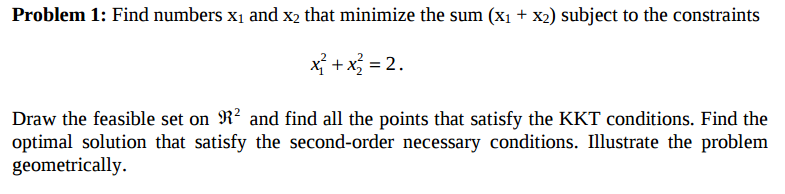
\includegraphics[width=0.7\linewidth]{screenshot001}
\label{fig:screenshot001}
\end{figure}

According to the task description, we will show the formula of the \textit{c(x)}:
\begin{flalign*}
c(x) = x_1^2 + x_2^2 -2 = 0
\end{flalign*}

The lagrangian function is ($\lambda$ is the lagrangian multiplier):
\begin{flalign*}
L(x, \lambda) = f(x) - \lambda c(x) = x_1 + x_2 - \lambda(x_1^2 + x_2^2 - 2)
\end{flalign*}

Now we will formulate the KKT conditions for the given system:
\begin{flalign*}
\frac{\delta L(x,\lambda)}{\delta x_1} = 1-\lambda x_1 \triangleq 0,\ then\  x_1 = \frac{1}{2\lambda}\\
\frac{\delta L(x,\lambda)}{\delta x_2} = 1-\lambda x_1 \triangleq 0,\ then\  x_2 = \frac{1}{2\lambda}
\end{flalign*}
The c(x) function, subject to calculated x, shall be zero:
\begin{flalign*}
x_1^2 +x_2^2 -2 = 0\\
(\frac{1}{2\lambda})^2 + (\frac{1}{2\lambda})^2 -2 = 0\\
\\
\lambda^2 = \frac{1}{4}
\\
\lambda = \frac{1}{2} \lor \lambda = -\frac{1}{2}
\end{flalign*}
Now we are calculating both $x_1\ and\ x_2$ according to lambda:
\begin{flalign*}
x = \begin{bmatrix}
1\\
1
\end{bmatrix}\\
x = \begin{bmatrix}
-1\\
-1
\end{bmatrix}
\end{flalign*}

Now to establish the min condition:
\begin{flalign*}
\min_x \{x_1+x_2\}\\
\\
for x = \begin{bmatrix}
1\\
1
\end{bmatrix}&:x_1+x_2 = 2\\
for x = \begin{bmatrix}
-1\\
-1
\end{bmatrix}&:x_1+x_2 = -2\\
\\
\end{flalign*}
Hence, the solution is:
$x = \begin{bmatrix}
-1\\
-1
\end{bmatrix}$

\begin{figure}[h]
\centering
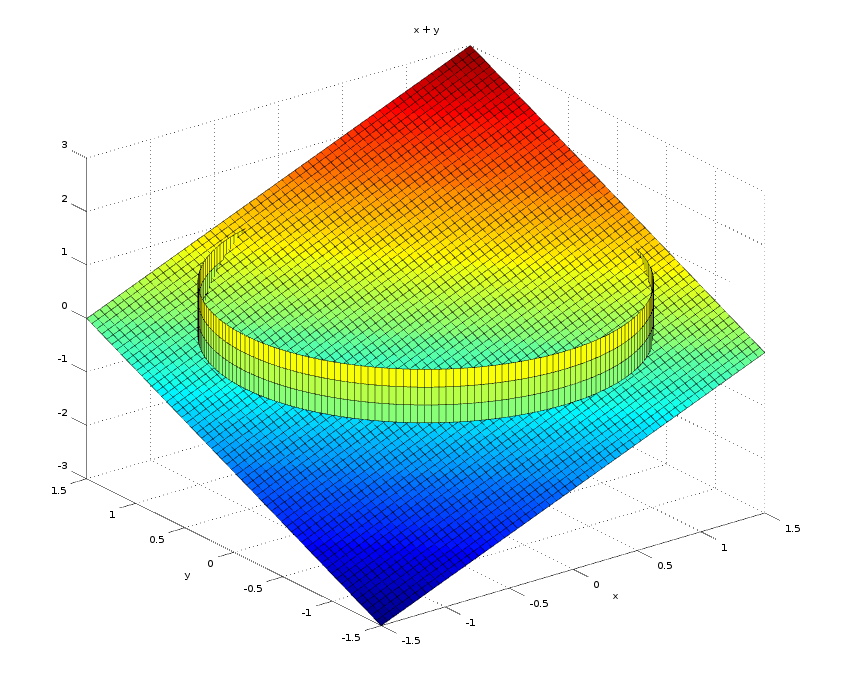
\includegraphics[width=0.7\linewidth]{screenshot002}
\caption{The graphical interpretation of given problem (cylinder of radius $\sqrt2)$ and the plane x+y ($x_1 + x_2$). The solution is in point [-1,-1] - the lowest point in Z-axis that is intersection of the mentioned two surfaces.}
\label{fig:screenshot002}
\end{figure}

The following code was used to illustrate the problem:
\begin{lstlisting}
pkg load symbolic

syms x y;

ezsurf (@(x, y) x + y, [-1.5 1.5 -1.5 1.5])
hold
[X, Y, Z] = cylinder([sqrt(2) sqrt(2) sqrt(2) sqrt(2)],200);
surf(X,Y,Z); 

\end{lstlisting}
\clearpage

%task2
\begin{figure}[h]
\centering
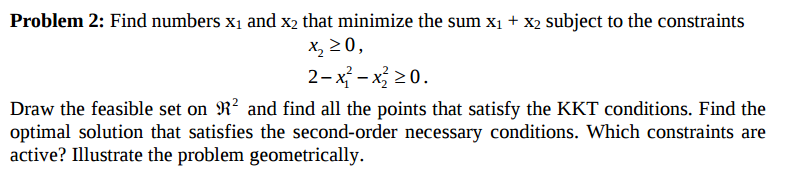
\includegraphics[width=0.7\linewidth]{screenshot003}
\label{fig:screenshot003}
\end{figure}
In the following task, we can distinguish two constrains:
\begin{flalign*}
f(x) = x_1 + x_2\\
c_1(x)=x_2 \geq 0\\
c_2(x)=2 - x_1^2 -x_2^2 \geq 0
\end{flalign*}
Therefor the Lagrangian form is:
\begin{flalign*}
L(x, \lambda) = f(x) - \lambda_1 c_1(x) - \lambda_2c_2(x) = x_1 + x_2 -\lambda_1x_2 - \lambda_2(2-x_1^2-x_2^2)
\end{flalign*}
Calculation for the following KKT conditions:
\begin{flalign*}
\frac{\delta L(x,\lambda)}{\delta x_1} = 1-2\lambda_2 x_1 \triangleq 0,\ then\  x_1 = \frac{1}{2\lambda_2}\\
\\
\frac{\delta L(x,\lambda)}{\delta x_2} = 1-\lambda x_1 \triangleq 0,\ then\  x_2 = \frac{\frac{1-\lambda_1}{2\lambda_2}}{den}
\end{flalign*}
We can treat inequalities as "equal to zero":
\begin{flalign*}
2 - (\frac{1}{2\lambda_2})^2 - (\frac{1-\lambda_1}{2\lambda_2})^2 = 0\\
\frac{1-\lambda_1}{2\lambda_2} = 0\\
\\
\lambda_1 = 1\\
\lambda_2^2 = 1/8,\ so\ \lambda_2  = \frac{1}{2\sqrt2} \lor -\frac{1}{2\sqrt2}
\end{flalign*}
After substituting lambda, we calculating the x (we obtain two variants):
\begin{flalign*}
x_a = [x_1\ x_2] &= [\ \ \sqrt2\ \ 0]\\
&\lor\\
x_b = [x_1\ x_2] &= [-\sqrt2\ \ 0]\\
\end{flalign*}
Point $x_b$ is a solution
\begin{figure}[h]
\centering
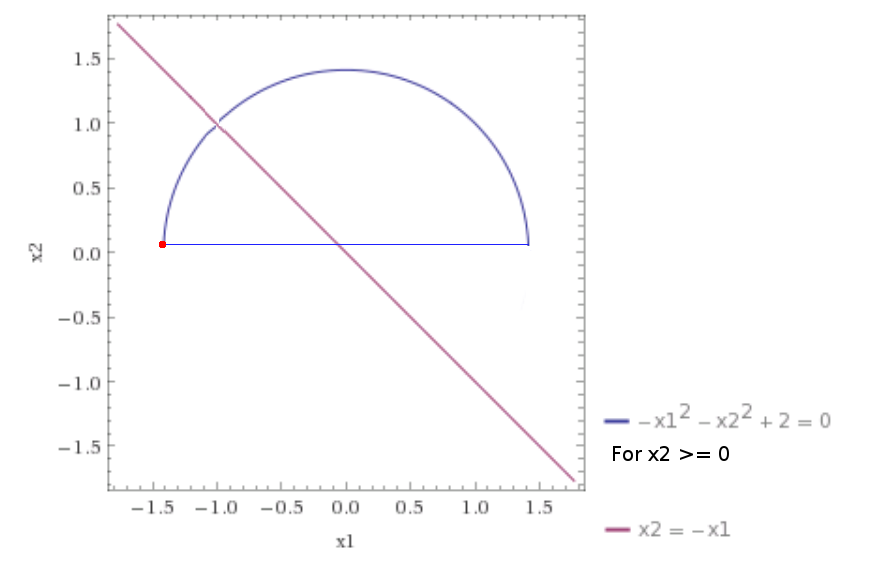
\includegraphics[width=0.9\linewidth]{screenshot004}
\caption{Graphical representation. The solution is the point below the line and inside the circle half (including edges).
In this case it is the point the most at the bottom left.}
\label{fig:screenshot004}
\end{figure}

\clearpage 

%task3
\begin{figure}[h]
\centering
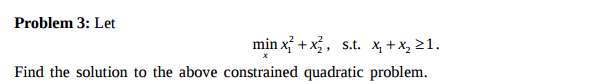
\includegraphics[width=0.7\linewidth]{screenshot005}
\label{fig:screenshot005}
\end{figure}
The problem can be easily solved using analytic geometry.
The minimization problem represents a circle of unknown radius, while the constraint is a semi--surface, but we can assume it as a line.
\begin{figure}[h]
\centering
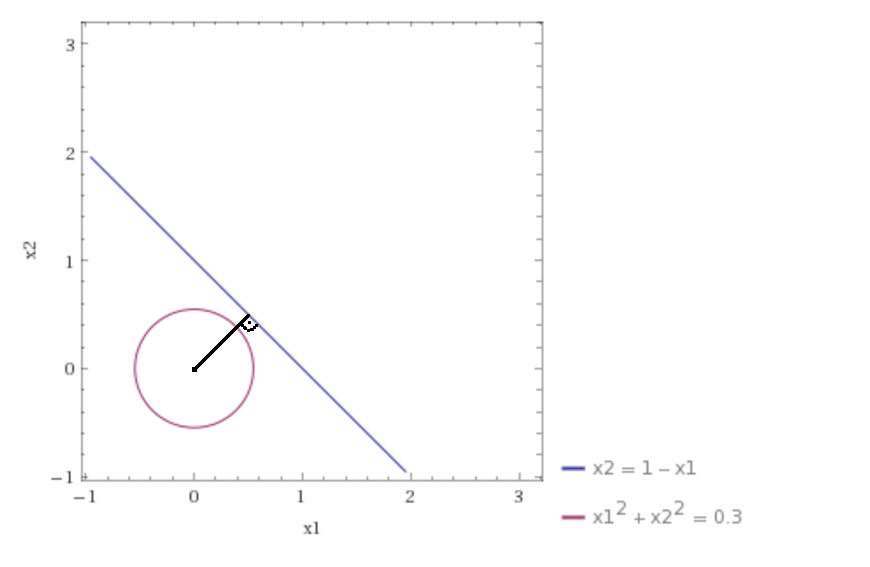
\includegraphics[width=0.7\linewidth]{screenshot006}
\caption{The solution will be a point lying on the line, which is tangent to unknown circle of radius R (circle on the figure is just example).}
\label{fig:screenshot006}
\end{figure}
Looking at first line equation, we can deduct that perpendicular line will have first coefficient equal to $a = 1$. So the thing is just to calculate the free coefficient.\\
However we know that certainly it has to go straight through the circle center (0,0).
Therefore the free coefficient $b = 0$
The two lines line has the form
\begin{flalign*}
x_2 = 1 - x_1
x_{2p} = x_{1p}
\end{flalign*}
The point they cross, is the solution. After solving this problem, we obtain:
\begin{flalign*}
x = [x_1\ x_2] = [\frac{1}{2},\ \frac{1}{2}]=[0.5,\ 0.5]
\end{flalign*}
\clearpage




%task5
\begin{figure}[h]
\centering
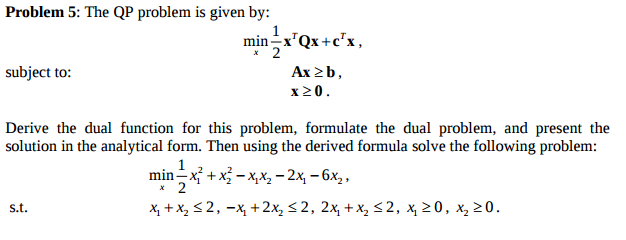
\includegraphics[width=0.7\linewidth]{screenshot007}
\label{fig:screenshot007}
\end{figure}
The problem will be solved using Quadratic Programming.
\\
To prepare the data for algorithms, we need to calculate the A,b Q and c matrices.
\\
Matrix A and c are based on given constraints:
\begin{flalign*}
A = 
\begin{bmatrix}
1  & 1\\
-1 & 2\\
2  & 1
\end{bmatrix},\ 
b = 
\begin{bmatrix}
2\\2\\2
\end{bmatrix}
\end{flalign*}

The next step is to calculate the matrices Q and c. They can be formulate by looking at the general form of the formula:
\begin{flalign*}
f(x) &= \frac{1}{2}q_{11}x_1^2 + \frac{1}{2}q_{22}x_2^2 + 
q_{12}x_1x_2 + 
c_1x_1 + c_2x_2\\
\\
f(x) &= \frac{1}{2}x_1^2 + \frac{1}{2}x_2^2 - 
x_1x_2 + 
-2x_1 -6x_2\\
\\
Q &= 
\begin{bmatrix}
1  & -1\\
-1 & 2\\
\end{bmatrix},\ 
c = 
\begin{bmatrix}
-2\\
-6
\end{bmatrix}
\end{flalign*}

\begin{lstlisting}
QP range
x =
0.45714
1.25714

Elapsed time is 0.00281096 seconds.


QP conjugacy
x =
0.45714
1.25714

Elapsed time is 0.00119114 seconds.
\end{lstlisting}
\clearpage


%task6
\begin{figure}[h]
\centering
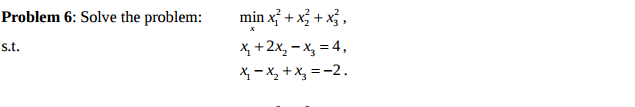
\includegraphics[width=0.7\linewidth]{screenshot008}
\label{fig:screenshot008}
\end{figure}
Based on the given data, the following data was prepared:
\begin{figure}[h]
\centering
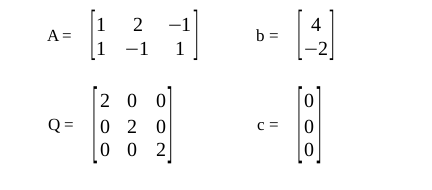
\includegraphics[width=0.55\linewidth]{screenshot010}
\label{fig:screenshot010}
\end{figure}

and Octave code was coded to solve this task:
\begin{lstlisting}
A = [1 2 -1; 1 -1 1 ]
b = [4; -2]

Q = [2 0 0; 0 2 0; 0 0 2]
c = [0;0;0]

tic
x = QP_range(A,b,Q,c)
toc

tic
x = QP_conjugacy(A,b,Q,c)
toc
\end{lstlisting}

The computations were made and there are the results. This time the QP range-space method was faster:
\begin{lstlisting}
QP range
x =
0.28571
1.42857
-0.85714

Elapsed time is 0.000784874 seconds.


QP conjugacy
x =
0.28571
1.42857
-0.85714

Elapsed time is 0.00107598 seconds.
>>
\end{lstlisting}
\clearpage



%task7
\begin{figure}[h]
\centering
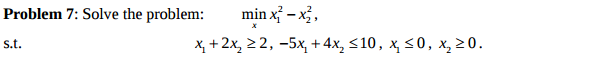
\includegraphics[width=0.7\linewidth]{screenshot009}
\label{fig:screenshot009}
\end{figure}
Once again, the matrices was prepared in order to start the algorithm:
\begin{flalign*}
A &= 
\begin{bmatrix}
1  & 2\\
5 & -4\\
\end{bmatrix},\ 
b = 
\begin{bmatrix}
2\\-10
\end{bmatrix}
\\
\\
Q &= 
\begin{bmatrix}
2  & 0\\
0 & 2\\
\end{bmatrix},\ 
c = 
\begin{bmatrix}
0\\
0
\end{bmatrix}
\end{flalign*}
The matlab code construction is exactly the same as in previous task, only the data changes.
\begin{lstlisting}
QP range
x =
-0.85714
1.42857

Elapsed time is 0.000548124 seconds.



QP conjugacy
x =
-0.85714
1.42857

Elapsed time is 0.000355005 seconds.
\end{lstlisting}
\clearpage








\clearpage
\chapter{Listings of algorithms}
Algorithm 1 - QP range--space\\ 
\begin{lstlisting}
function [x_sol] = QP_range(A,b,Q,c)
	disp("QP range")
	x = A\b;
	g = c+Q*x;
	r = A*x -b;
	invQ = inv(Q);
	lambda = (A*invQ*A')\(A*invQ*g-r);
	p= Q\(A'*lambda -g);
	x_sol = x + p;
endfunction
\end{lstlisting}

Algorithm 2 - QP Conjugacy based\\
\begin{lstlisting}
function [x_sol] = QP_conjugacy(A,b,Q,c)

	disp("QP conjugacy")
	
	x = A\b;
	g = c+Q*x;
	r = A*x -b;
	
	[Qa, Ra] = qr(A');
	L = chol(Qa'*Q*Qa);
	
	W = Qa*inv(L);
	[m,n] = size(W);
	
	Z = W(1:end, 1:n-m);
	Y = W(1:end, n-m+1:end);
	
	py = (A*Y)\(-r);
	pz = -Z'*g;
	p = Y*py + Z*pz;
	
	x_sol = x + p;
endfunction
\end{lstlisting}
\begin{thebibliography}{8}
\addcontentsline{toc}{chapter}{Bibliography}
%\addcontentsline{toc}{section}{Literatura}
\bibitem{nocedal}
J. Nocedal, S. J. Wright, Numerical Optimization, Springer, 1999,
\bibitem{zdunek}
Zdunek R., Optimization Methods - lecture slides.
\bibitem{mathworks}
Methods for Constrained Optimization,
Coralia Cartis, University of Oxford
\end{thebibliography}

\end{document}

